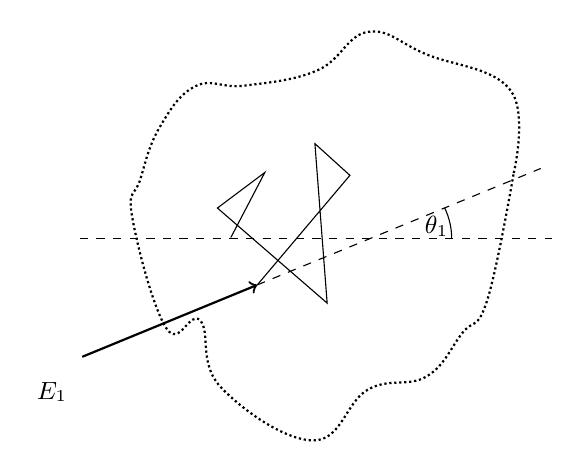
\begin{tikzpicture}[scale=0.6]

	% Dashed reference lines to show angles
	\draw[dashed] (-5.05,-0.5) -- ++(10,0);

	% Supernova Remnant
	\draw[densely dotted, thick] 
	plot[smooth, tension=0.7] 
	coordinates {
		(4.134,0.891)
		(4.071,2.634)
		(2.285,3.402)
		(1.052,3.878)
		(-0.016,3.066)
		(-1.558,2.741)
		(-2.596,2.731)
		(-3.356,1.867)
		(-3.770,0.759)
		(-3.940,-0.056)
		(-3.217,-2.399)
		(-2.503,-2.231)
		(-2.075,-3.634)
		(-0.119,-4.770)
		(1.043,-3.696)
		(2.288,-3.416)
		(3.043,-2.499)
		(3.573,-1.799)
		(4.134,0.891)
	};


	% Incoming particle E1
 	\draw[->, thick] (-5, -3) -- (-1.295,-1.478) 
	node[pos=0.1, below left=8pt] {\small $E_1$};
	\draw[dashed] (-1.295, -1.478) -- ++(6,2.4648); % reference for theta_1
	\draw (1.320,-0.5) +(0:1.5) arc[start angle=0, end angle=26, radius=1.5];
	\node at (2.50,-0.24) {\small $\theta_1$};





	% Outgoing particle E2
	%\draw[->, thick] (-1.5, -1.5) -- (-4, -0.8) node[midway, below left=-2pt] {\small $E_2$};

	% Velocity vector V (leftward, from scattering point)
	%\draw[->, thick] (2.5, 2.0) -- (0.5, 2.0) node[midway, above] {\small $\vec{V}$};

	% Dashed reference lines to show angles
	%\draw[dashed] (2.5,2.0) -- ++(2,0); % reference for theta_1
	%\draw[dashed] (2.5,2.0) -- ++(-2,2); % reference for theta_2

	% Angle arcs
	%\draw (2.5,2.0) +(0:1.0) arc[start angle=0, end angle=135, radius=1.0];
	%\node at (1.9,2.9) {\small $\theta_2$};

	%\draw (2.5,2.0) +(0:0.7) arc[start angle=0, end angle=-45, radius=0.7];
	%\node at (3.1,1.5) {\small $\theta_1$};

	% scatter path
	\draw plot coordinates {
	(-1.854, -0.474)
	(-1.134,0.903)
	(-2.138,0.149)
	(0.184,-1.863)
	(-0.075,1.512)
	(0.666,0.841)
	(-1.295,-1.478)
	};

\end{tikzpicture}
